\section{Documentation Testing}
\label{sec:Documentation Testing}

\rindex{\textbf{D}!Documentation Testing}A confusing term. There are no reason for test the documentation. Use it in testing, that's all!

Just grab \rindex{\textbf{R}!Requirements}requirements and think:
\begin{itemize}
 \item what should be implemented,
 \item what can be tested.
\end{itemize}

\begin{figure}[!h]
\centering
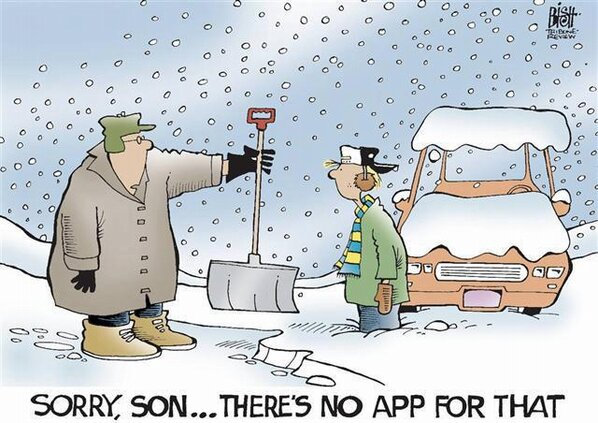
\includegraphics[width=0.8\linewidth]{no-app-for-that}
\caption{\ttfamily{'Sorry, son\ldots there's no app for that'}}
\label{fig:no-app-for-that}
\end{figure}

You will need only \rindex{\textbf{N}!Notepad} Notepad and your own imagination for this.

Note all your ideas and questions, search for answers, and repeat steps one by one (this is an incremental task) till the end of your career in testing.
